
\definecolor{cc6c6c6}{RGB}{198,198,198}
\definecolor{cffffff}{RGB}{255,255,255}

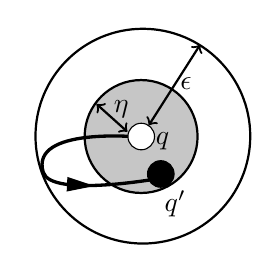
\begin{tikzpicture}[y=0.4pt, x=0.4pt,yscale=-1, inner sep=0pt, outer sep=0pt]
% path5273
\path[shift={(-0.42857142,4.7142857)},draw=black,miter limit=4.00,line
  width=0.800pt]
  (365.7143,269.5050)arc(0:180:97)arc(-180:0:97) --
  cycle;

% path5275
\path[shift={(-6.0609153,-3.535534)},draw=black,fill=cc6c6c6,miter
  limit=4.00,line width=0.800pt]
  (323.7539,278.0803)arc(-0:180:51)arc(-180:0:51) --
  cycle;

% path5315
\path[draw=black,line join=miter,line cap=butt,miter limit=4.00,line
  width=1.200pt] (265.6701,275.0498) .. controls (265.6701,275.0498) and
  (165.7228,265.2948) .. (178.2919,306.8696) .. controls (185.4208,330.4496) and
  (285.8732,311.9204) .. (285.8732,311.9204) -- (285.8732,311.9204);

% path4761
\path[draw=black,fill=cffffff,miter limit=4.00,line width=0.400pt]
  (278.8021,274.5447)arc(0:180:12)arc(-180:0:12) --
  cycle;

% path4761-4
\path[shift={(17.677674,33.840124)},draw=black,fill=black,miter limit=4.00,line
  width=0.400pt]
  (278.8021,274.5447)arc(-0:180:12)arc(-180:0:12) --
  cycle;

% text5307
\path[fill=black] (288,334.92981) node[right] (text5307) {$q'$};

% text5311
\path[fill=black] (280,286.9537) node[above right] (text5311) {$q$};

% path5319
\path[draw=black,fill=black,line join=miter,line cap=butt,line width=0.800pt]
  (201.0204,312.4254) -- (220.7183,318.9914) -- (200.5153,323.0320) --
  (201.0204,312.4254) -- cycle;

% path2829
\path[draw=black,line join=miter,line cap=butt,line width=0.800pt,<->]
  (273.5714,264.5050) -- (320.0,191.6479);

% path2831
\path[draw=black,line join=miter,line cap=butt,line width=0.800pt,<->]
  (254.2857,270.2193) -- (226.4286,245.2193);

% text2833
\path[fill=black] (302.14285,231.6479) node[above right] (text2833) {$\epsilon$};

% text2837
\path[fill=black] (242.14285,258.07648) node[above right] (text2837) {$\eta$};


\end{tikzpicture}
